\section{Result}

\begin{enumerate}
    \item Calculate the separations of the planes (111), (211), and (100) in a crystal in which the simple cubic unit cell has the side \( a = 0.432 \, \text{nm} \).
    \item From Bragg’s equation, what is the minimum d-spacing that can be observed with a wavelength of \( 0.07 \, \text{nm} \)? What do you need in order to observe smaller d spacings?
    \item Reflection from the (111) planes of a cubic crystal was observed at an incident angle \( \theta = 11.2^\circ \) when Cu K\(\alpha\) X-rays of wavelength \( 0.154 \, \text{nm} \) were used. What is the length of the side of the unit cell?
    \item Calcium carbonate crystals in the form of aragonite have an orthorhombic unit cell with dimensions \( a = 0.574 \, \text{nm} \), \( b = 0.796 \, \text{nm} \), \( c = 0.495 \, \text{nm} \). Calculate the incident angles for the (100), (010), and (111) reflections using radiation of wavelength \( 0.083 \, \text{nm} \).
    \item Calculate the allowed values of \( hkl \) for a body-centered cubic (bcc) and face-centered cubic (fcc) system that will give Bragg points on a diffraction pattern.
    \item Find the two elements.
    \item Measure the full width at half maximum (FWHM) of each peak of the two diffraction patterns and calculate the crystallite size using Scherrer’s equation. Scherrer’s equation is suitable for particle sizes below approximately \( 100 \, \text{nm} \). Which property of light limits this kind of quantification? 
    \begin{itemize}
        \item \textbf{Hint:} Constructive interference of two waves (and therefore diffraction) does not happen with any kind of light.
    \end{itemize}
    Bragg’s law is based on the ideal case where a strictly monochromatic source is used. However, every X-ray source has a certain finite spectral bandwidth, \( \frac{\Delta \lambda}{\lambda} \). As a result, the broader the spectral bandwidth, the broader the diffraction peaks.
    
    \item[(a)] Prove that the spectral contribution of the source to the peak width, \( \Delta \theta \), is related to the spectral bandwidth through the following relation:
    \[
    \Delta \theta = \tan \theta \frac{\Delta \lambda}{\lambda} \quad (9.2)
    \]
    \textbf{Hint:} Differentiate Bragg’s law.

    \item[(b)] Although this contribution affected the estimation you made in Exercise 7, it can be quantified to obtain a more exact crystallite size. Can you think of at least one other phenomenon or instrumental property that can affect the peak widths?
\end{enumerate}

\begin{figure}[H]
    \centering
    \begin{subfigure}[b]{0.99\textwidth} 
        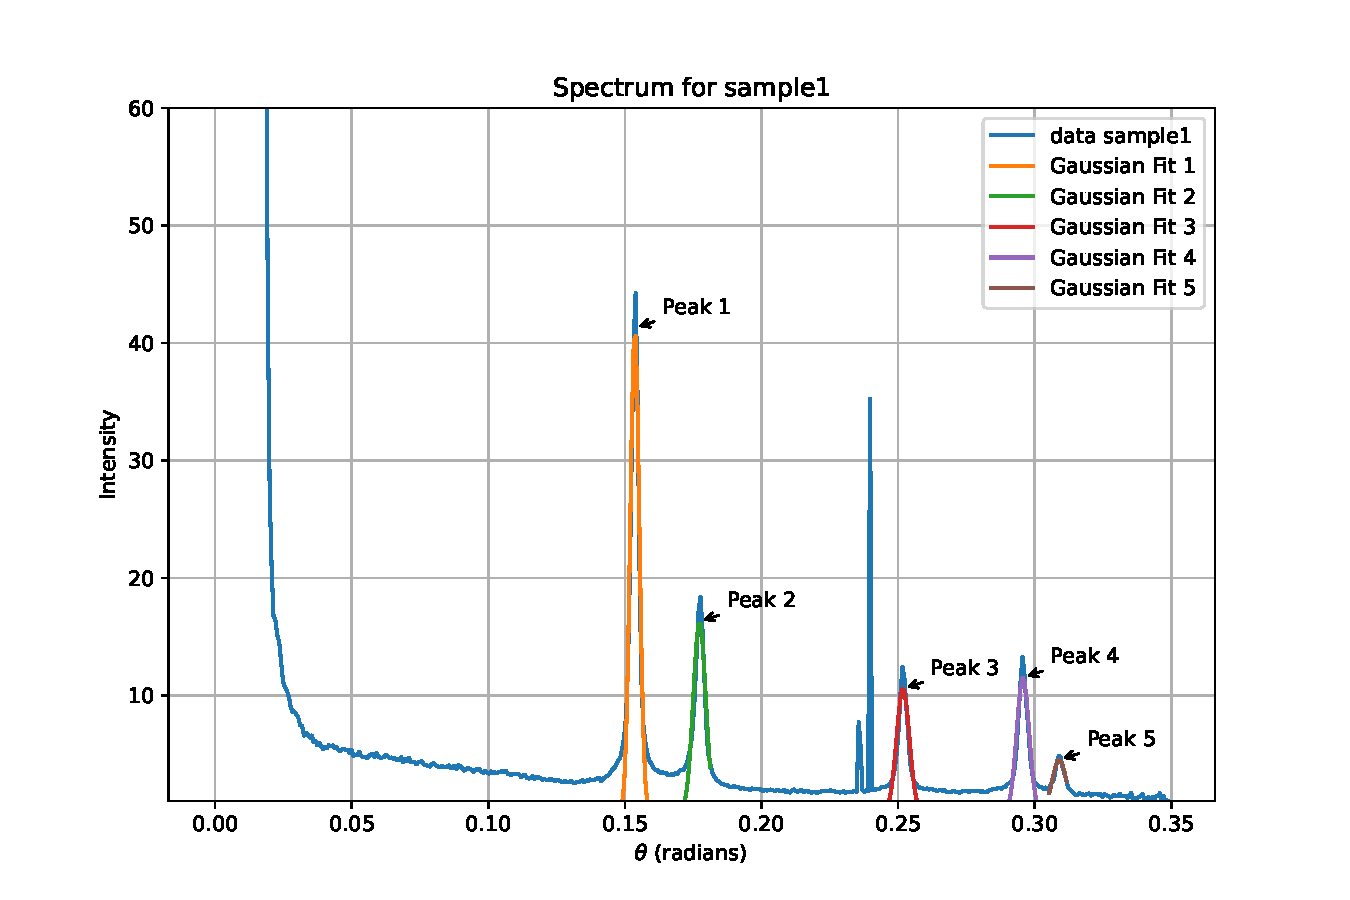
\includegraphics[width=\textwidth]{Figures/gaussian_sample1.pdf}
        \subcaption{This is the first subfigure.}
        \label{fig:subfigure1}
    \end{subfigure}
    \begin{subfigure}[b]{0.99\textwidth} 
        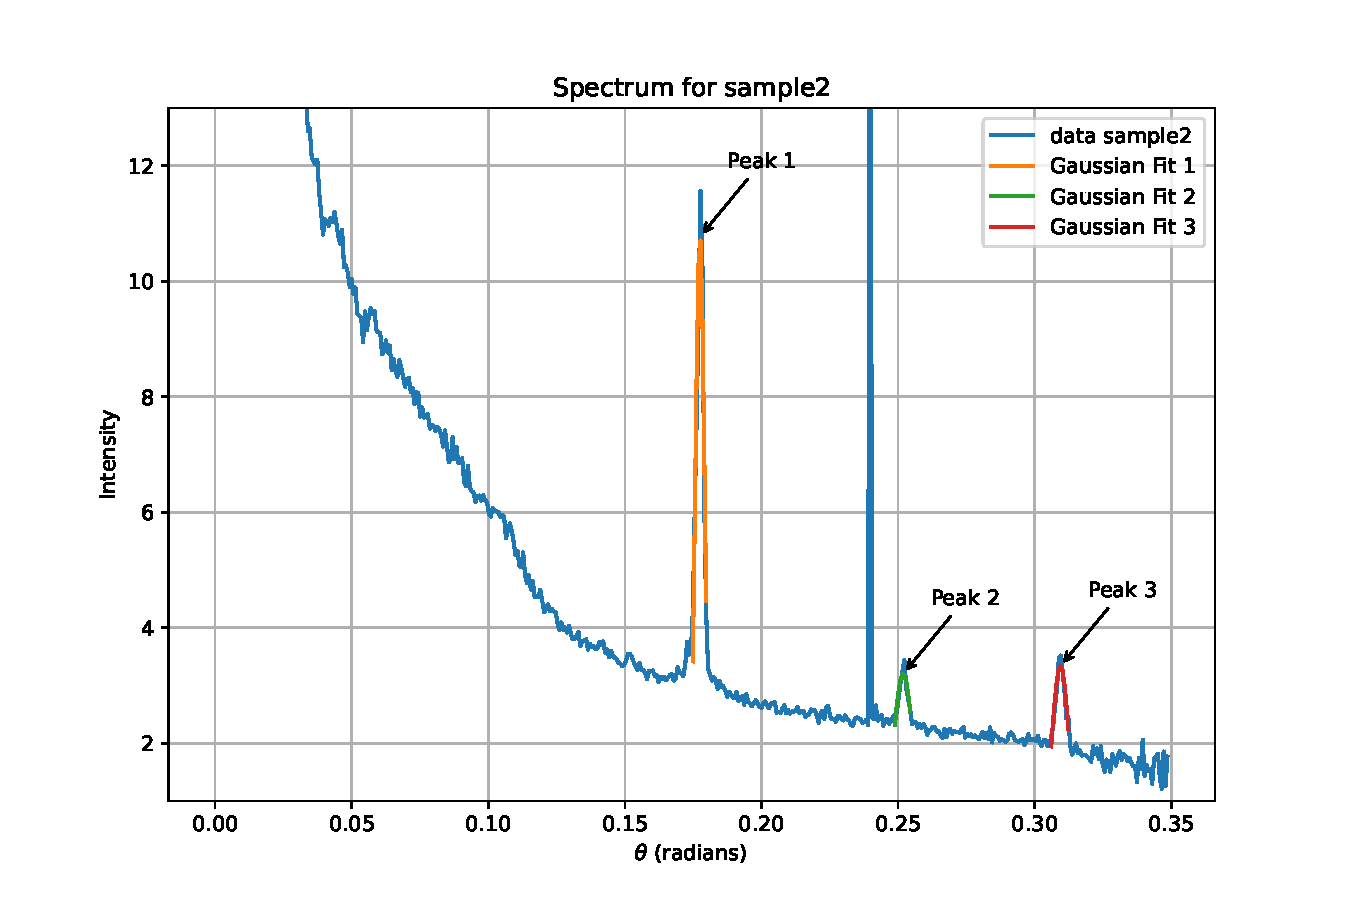
\includegraphics[width=\textwidth]{Figures/gaussian_sample2.pdf}
        \subcaption{This is the second subfigure.}
        \label{fig:subfigure2}
    \end{subfigure}
    \caption{This figure shows two subfigures with separate captions.}
    \label{fig:result_figure}
\end{figure}

\begin{table}[H]
    \centering
    \caption{Fitting results for Sample 1}
    \begin{tabular}{|c|c|c|c|}
    \hline
    Peak & Amplitude & Mean & FWHM \\
    \hline
    Peak 1 & \SI{41.29(2.15)}{units} & \SI{0.15362(0.00010)}{radians} & \SI{0.00388(0.00023)}{radians} \\
    \hline
    Peak 2 & \SI{16.28(1.14)}{units} & \SI{0.17731(0.00019)}{radians} & \SI{0.00535(0.00046)}{radians} \\
    \hline
    Peak 3 & \SI{10.57(0.71)}{units} & \SI{0.25180(0.00018)}{radians} & \SI{0.00550(0.00043)}{radians} \\
    \hline
    Peak 4 & \SI{11.53(0.66)}{units} & \SI{0.29569(0.00015)}{radians} & \SI{0.00530(0.00035)}{radians} \\
    \hline
    Peak 5 & \SI{4.51(0.19)}{units} & \SI{0.30900(0.00015)}{radians} & \SI{0.00616(0.00049)}{radians} \\
    \hline
    \end{tabular}
\end{table}

\begin{table}[H]
    \centering
    \caption{Fitting results for Sample 2}
    \begin{tabular}{|c|c|c|c|}
    \hline
    Peak & Amplitude & Mean & FWHM \\
    \hline
    Peak 1 & \SI{10.77(0.62)}{units} & \SI{0.17746(0.00012)}{radians} & \SI{0.00404(0.00034)}{radians} \\
    \hline
    Peak 2 & \SI{3.20(0.09)}{units} & \SI{0.25186(0.00017)}{radians} & \SI{0.00895(0.00092)}{radians} \\
    \hline
    Peak 3 & \SI{3.34(0.10)}{units} & \SI{0.30942(0.00014)}{radians} & \SI{0.00768(0.00056)}{radians} \\
    \hline
    \end{tabular}
\end{table}
